\usetikzlibrary{shapes.arrows,chains}
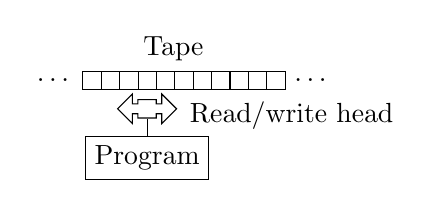
\begin{tikzpicture}[
      start chain=1 going right,start chain=2 going below,node distance=-0.15mm
    ]
    \node [on chain=2] {Tape};
    \node [on chain=1] at (-1.5,-.4) {\ldots};
    \foreach \x in {1,2,...,11} {
        \x, \node [draw,on chain=1] {};
    }
    \node [name=r,on chain=1] {\ldots};
    \node [name=k, arrow box, draw,on chain=2,
        arrow box arrows={east:.25cm, west:0.25cm}] at (-0.335,-.65) {};
    \node at (1.5,-.85) {Read/write head};
    \node [on chain=2] {};
    \node [draw,on chain=2] {Program};
    \chainin (k) [join]; % Verbindung vom Programm zum Leseschreibkopf
\end{tikzpicture}
